\documentclass[xetex,mathserif,serif]{beamer}

\usepackage[log-declarations=false]{xparse}
\usepackage[quiet]{fontspec}
\usepackage{amsmath}
\usepackage{amsfonts}
\usepackage{mathtools}
\usepackage{enumerate}
\usepackage{polyglossia}
\usepackage{tikz}
\usepackage{unicode-math}
\usetikzlibrary{arrows,shapes,trees}

\newcommand{\vank}{\emph{Seifert-van Kampen} }

% works for now
\setbeamertemplate{footline}{\insertframenumber/\inserttotalframenumber}

\setdefaultlanguage{spanish}

\begin{document}

  \begin{frame}
    \begin{center}
      \begin{block}{}
        Topología Algebraica
      \end{block}
      \begin{block}{}
        Ruben Astudillo
      \end{block}
    \end{center}

  \end{frame}

  \begin{frame}
    \frametitle{Motivación}

    \begin{block}{}
      Definir una invariante para espacios topológicos.
    \end{block}

    \pause

    \begin{block}{}
      Idea: Estudiar las curvas y las ``deformaciones'' admisibles entre
      ellas para un espacio dado.
    \end{block}
  \end{frame}

  \begin{frame}
    \frametitle{Curvas y homotopias}
    \begin{columns}

      \begin{column}{.5\textwidth}
        \begin{center}
          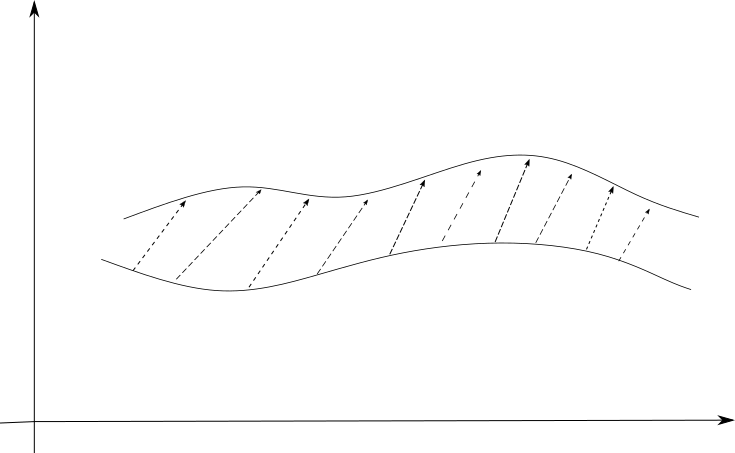
\includegraphics[scale=0.3]{../tesis/imagenes/homotopia.png}
        \end{center}
      \end{column}

      \pause

      \begin{column}{.5\textwidth}
        \begin{block}{Camino}
          Es una función continua \[ f : I \to X \] con \(X\) un espacio
          topológico
        \end{block}

        \pause

        \begin{block}{Homotopía entre \(f\) y \(g\)}
          Es una función continua \(H : I \times I \to X\) tal que
          \[ H(x,0) = f(x),\ H(x,1) = g(x) \]
          \[ f \sim g \]
        \end{block}
      \end{column}
    \end{columns}
  \end{frame}

  \begin{frame}
    \frametitle{Producto de caminos y homotopias}
    Si \(f (1) = g (0) \in X\) entonces el producto de caminos esta
    definido por
    \[ f * g (t) :=
      \begin{cases}
        f(2t) & t \in [0, \frac 1 2] \\
        g(2t - 1) & t \in [\frac 1 2 , 1 ]
      \end{cases}
    \]

    \begin{center}
      \begin{tikzpicture}[scale=0.8]
        \draw [blue, thick]  (0,0) to[bend right] (3,2) to[bend left] (4,3) ;
        \draw [red, thick] (4,3) to[bend right] (9,1) ;
      \end{tikzpicture}
    \end{center}

    \pause

    \begin{block}{}
      En general se consideran curvas con el mismo punto inicial y final
      (caminos cerrados).
    \end{block}
  \end{frame}

  \begin{frame}
    \frametitle{Producto de caminos y homotopias}
    Análogamente para homotopias \(F\) y \(G\) tal que \(H(1, t) =
    G(0,s) , \forall s, t \in I\), se define el producto de homotopias
    \[ F * G (x, t) :=
      \begin{cases}
        F(x, 2t) & t \in [0, \frac 1 2] \\
        G(x, 2t - 1) & t \in [\frac 1 2, 1]
      \end{cases}
    \]

    \begin{center}
      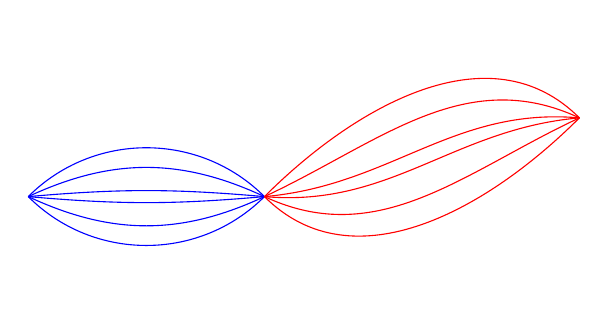
\begin{tikzpicture}
        \draw[blue] (0,1) to[out=45, in=135] (3,1) ;
        \draw[blue] (0,1) to[out=25, in=155] (3,1) ;
        \draw[blue] (0,1) to[out=5, in=175] (3,1) ;
        \draw[blue] (0,1) to[out=-5, in=185] (3,1) ;
        \draw[blue] (0,1) to[out=-25, in=205] (3,1) ;
        \draw[blue] (0,1) to[out=-45, in=225] (3,1) ;

        \draw[red] (3,1) to[out=45, in=135] (7,2) ;
        \draw[red] (3,1) to[out=25, in=155] (7,2) ;
        \draw[red] (3,1) to[out=5, in=175] (7,2) ;
        \draw[red] (3,1) to[out=-5, in=185] (7,2) ;
        \draw[red] (3,1) to[out=-25, in=205] (7,2) ;
        \draw[red] (3,1) to[out=-45, in=225] (7,2) ;
      \end{tikzpicture}
    \end{center}
  \end{frame}

  \begin{frame}
    \frametitle{Grupo fundamental}
    \begin{block}{}
      Todo camino \(f : I \to X\) tiene un camino inverso \(\overline f (t)
      := f( 1 - t)\)
    \end{block}
    \begin{block}{}
      Se define el conjunto
      \[ \pi (X, x_0) := \{ [f] \mid f : I \to X ,\ f(0) = f(1) = x_0
        \} \]
      \[ [f] * [g] := [f * g]\]
      \[ g \in [f] \iff f \simeq g ,\ \text{ie existe una homotopía
          entre ellos}\]
    \end{block}

    \begin{block}{}
      La tupla \(
      \left(\pi(X, x_0), (*) \right) \) es llamado el grupo fundamental de \(X\).
    \end{block}
  \end{frame}

  \begin{frame}
    \frametitle{Importancia punto de origen}
    \begin{block}{}
      Esta invariante es útil en general solo para espacios arco-conexo
      pues queremos que la elección de punto \(x_0\) no afecte al grupo.
    \end{block}

    \pause

    \begin{block}{}
      El punto de origen igual se incluye por la caracterización de
      conmutatividad del grupo fundamental y tratamiento mas explicito con
      respecto a la teoría de cubrimientos.
    \end{block}
  \end{frame}

  \begin{frame}
    \frametitle{El grupo fundamental es una invariante}
    Si \(f : (X, x) \to (Y, y) \) es un homeomorfismo, \[¿\pi (X, x)
    \simeq \pi (Y,y)?\]

    \pause

    Si, se define un isomorfismo por
    \begin{align*}
      f_* : \pi (X,x) &\to \pi (Y, y) \\
      [\gamma] &\longmapsto [ f \circ \gamma ]
    \end{align*}

    \pause

    Esta construccion es un homomorfismo para cualquier \(f\) continuo.
    Luego hemos construido realmente un functor entre \(\text{Top}_*
    \to \text{Grp}\)
  \end{frame}

  % Seccion ejemplo R^2 sin punto
  \begin{frame}
    \frametitle{Ejemplo intuitivo \(R^2\) menos un punto}
    \begin{figure}[h]
      \centering
      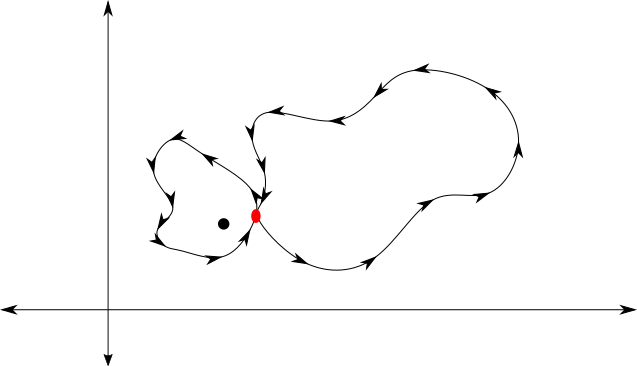
\includegraphics[scale=0.5]{../tesis/imagenes/R2-punto.png}
      \caption{\(R^2\) sin el punto \((1,1)\) en negro. Origen en rojo. }
    \end{figure}

  \end{frame}

  \begin{frame}
    \frametitle{Tres grandes herramientas de calculo}
    \begin{itemize}
    \item Retracciones y tipos homotopicos
    \item Teoria de cubrimientos
    \item Teorema de \vank
    \end{itemize}
  \end{frame}

  \begin{frame}
    \frametitle{Retracciones y tipos homotopicos}
    \begin{block}{Retraccion}
      Sea \(X\) un espacio topológico. El conjunto \(A \subset X\) es una
      retracción de \(X\) si existe un mapeo continuo \(r : X \to A\) tal que
      \[ r \mid_{A} (x) = x \]
      con \(r \mid_{A}\) siendo la restriccion de \(r\) al dominio \(A\). En
      caso de cumplirse esto, \(r\) es llamada la aplicación retracción de
      \(X\) en \(A\).
    \end{block}

    \begin{block}{Inclusion}
      Para toda retraccion \(A \subset X\), existe una funcion inclusion
      \[ j : A \to X \]
    \end{block}
  \end{frame}

  \begin{frame}
    \frametitle{Retracciones y tipos homotopicos}
    \begin{block}{Inyectividad grupos}
      Si \(A \subset X\) es una retracción, entonces la aplicación
      inclusión \(j : A \to X\) induce un homomorfismo de grupos
      fundamentales \(j_{*} : \pi(A, a) \to \pi(X,a)\) inyectivo para
      todo \(a \in A\).
    \end{block}
  \end{frame}

  \begin{frame}
    \frametitle{Retracciones y tipos homotopicos}

    \begin{block}{Lema}
      Sean \(h,k : (X, x_0) \to (Y, y_0)\) dos mapeos continuos. Si
      \(h\) y \(k\) son homotopicos y si la imagen de \(x_0\) bajo esta
      homotopía permanece fija en \(y_0\), entonces \(h_*\) e \(k_*\) son
      iguales.
    \end{block}
  \end{frame}

  \begin{frame}
     \frametitle{Retracciones y tipos homotopicos}
     \begin{block}{Inyectividad grupos}
       Si \(A \subset X\) es una retracción, entonces la aplicación
       inclusión \(j : A \to X\) induce un homomorfismo de grupos
       fundamentales \(j_{*} : \pi(A, a) \to \pi(X,a)\) biyectivo para
       todo \(a \in A\) si \(j \circ r\) homotopico a la identidad de \(X\).
     \end{block}
  \end{frame}

  \begin{frame}
    \frametitle{Tipos homotopicos}
    \begin{block}{Equivalencias homotopicas}
      Sean \(f : X \to Y\) e \(g : Y \to X\) mapeos continuos. Supongamos
      que \[ g \circ f \simeq Id : X \to X \]
      \[ f \circ g \simeq Id : Y \to Y \]
      Entonces \(f\) y \(g\) son llamadas \emph{equivalencias
      homotopicas} y la presencia de estas dicen que \(X,Y\) poseen el
      mismo grupo fundamental.
    \end{block}
  \end{frame}

  \begin{frame}
    \frametitle{Ejemplo de espacios mismo tipo homotopicos}
    \begin{block}{}
      \centering
      
\includegraphics{./imag/ThreeNonHomeoButHomotopyEquivGraphs.png}
    \end{block}

    \begin{block}{}
      \centering
      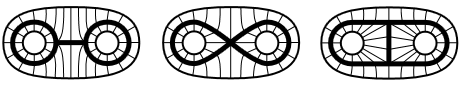
\includegraphics[scale=0.5]{./imag/HomotopyEquivalentsToBiAnnulus.png}
    \end{block}
    \begin{center}
      \emph{imagenes de Hatcher}
    \end{center}

  \end{frame}

  \begin{frame}
    \frametitle{Banda de Mobius}
    \centering
    \includegraphics[scale=0.3]{./imag/512px-MöbiusStripAsSquare.svg.png}
  \end{frame}

  \begin{frame}
    \frametitle{Categoria de homotopias}
    Se define una nueva categoria \(\mathscr{HoTop}_*\) correspondiente
    a la tripleta \(\left( \mathbf{Obj}, \mathbf{Mor}, (\circ) \right)\)
    con
    \begin{itemize}
    \item \(\mathbf {Obj}\) corresponde a espacio topologicos puntuados de la
      forma \((X, x_0)\).
    \item \(\mathbf {Mor}\) corresponde a un conjunto
      \[ \mathbf{Mor} = \{ [f] \mid f : (X,x_0) \to (Y,y_0),\
        (X,x_0),(Y,y_0) \in \mathbf {Obj} \}\]
      de clases equivalencias homotopicas entre funciones continuas.
    \item \((\hat \circ)\) corresponde a la composición de clases de
      equivalencias tal que si \([f] , [g] \in \mathbf {Mor} \) con
      \[ f : (X,x_0) \to (Y, y_0)\]
      \[ g : (Y, y_0) \to (Z, z_0)\]
      entonces \([g] \, \hat \circ \, [f] := [ g \circ f ] \) es una clase
      de equivalencia de funciones \((X, x_0) \to (Z, z_0)\).
    \end{itemize}
  \end{frame}
  \begin{frame}
    \frametitle{Categoria de homotopias}
    \begin{block}{Subcategoria Top}
      La categoria \(\mathscr{Top}_*\) se puede ver como una
      sub-categoria de \(\mathscr{HoTop}\) mediante el functor
      \[ i : \mathscr{Top}_* \to \mathscr{HoTop}_*\]
      mapeando los objetos a si mismos y tomando toda funcion continua
      \(f\) entre espacios vectoriales y asignandole \([f]\) en
      \(\mathscr{HoTop}\).

      Espacios topologicos biyectivos tiene claramente un par de
      equivalencias homotopicas!

      Se puede extender el functor \(\pi\) que asigna el grupo
      fundamental a un espacio topologico a trabajar desde
      \(\mathscr{HoTop}_* \to \mathscr{Grp}\)

      Muestra que la nocion de homeomorfismos era muy fuerte si la meta
      es clasificar espacios mediante el grupo fundamental.
    \end{block}
  \end{frame}

  \begin{frame}
    \frametitle{Pequeños resultados de esta homotopia}
    \begin{block}{Productos}
      Es una categoria cartesiana. El producto de espacios puntuados
      sera el producto catesiano usual \((X \times Y, (x_0, y_0))\). Mas
      aun, el functor \(\pi\) respetara la estructura del producto
      \[ \pi (X \times Y , (x_0, y_0)) = \pi (X, x_0) \times \pi (Y,
        y_0)\]
      siendo en la llegada el producto cartesiano de grupos. Este
      resultado se obtiene por la caracterizacion de curvas es un
      espacio producto.
    \end{block}
  \end{frame}
  \begin{frame}
    \frametitle{Pequeños resultados de esta homotopia}
    \begin{block}{Co-productos}
      Tambien tiene un co-producto por ser los objetos espacios
      puntuados. Para \((X, x_0) , (Y, y_0)\) se define el co-producto
      como
      \[ X \vee Y , \{x_0, y_0\} = X \sqcup Y / x_0 \simeq y_0 \]
    \end{block}
    \begin{block}{}
      ¿Preservara \(\pi\) la estructura del co-producto?
    \end{block}
  \end{frame}

  \begin{frame}
    \frametitle{Cubrimientos}
    \begin{columns}
      \begin{column}{0.3\textwidth}
        \centering
        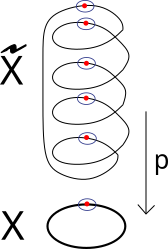
\includegraphics[scale=.8]{../tesis/imagenes/spring.png}
      \end{column}
      \begin{column}{0.7\textwidth}
        \begin{block}{Cubrimiento}
          \(p : \tilde{X} \to X\) una función continua sobreyectiva tal
          que para todo \(x \in X\) existe un abierto U y una familia
          \(\{V_\alpha\}_{\alpha \in \Lambda},\ \Lambda \subseteq \mathbb N\) tal
          que
          \[ p^{-1} (U) = \bigcup_{\alpha \in \Lambda} V_\alpha \]
          Donde \(\{V_\alpha\}\) es una familia disjunta de abiertos de
          \(\tilde X\), tal que
          la restriccion a cada \(V_\alpha\) de \(p\) es
          homeomorfa sobre \(U\).
        \end{block}
        \begin{block}{Fibra}
          Corresponde al conjunto de puntos en rojo.
          \[ p^{-1} \left( \{x_0\} \right) \]
        \end{block}
      \end{column}
    \end{columns}
  \end{frame}

  \begin{frame}
    \frametitle{Levantamiento de curvas al cubrimiento}
    \begin{columns}
      \begin{column}{.5\textwidth}
        \centering
        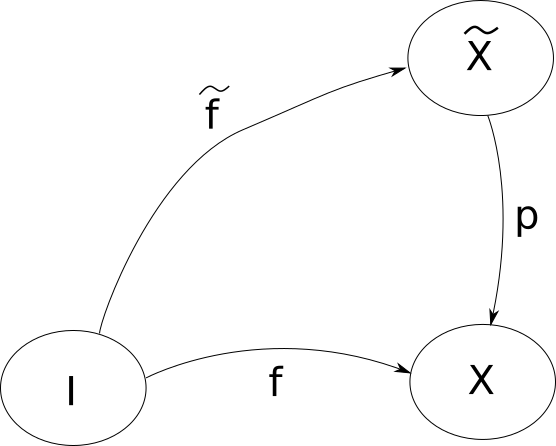
\includegraphics[scale=0.3]{../tesis/imagenes/lifting-path.png}
      \end{column}
    \begin{column}{.5\textwidth}

    \end{column}
    \end{columns}
  \end{frame}

\end{document}
